\documentclass{article}

\usepackage{geometry}
\geometry{letterpaper}

\usepackage{doc}

\usepackage{url}

\usepackage{graphicx}
\usepackage{epstopdf}
\DeclareGraphicsRule{.tif}{png}{.png}{`convert #1 `dirname #1`/`basename #1 .tif`.png}

\title{Headmaster Dream Design}
\author{Haley Young}
\date{\today}

\begin{document}

\maketitle

\pagebreak
\tableofcontents
\pagebreak

\section{Introduction}

When it comes to the Headmaster interface, the first thing that comes to mind is "boring". The purpose of this web service is to provide students with a way of looking up their academic information as well as provid the ability for teachers and faculty to look up information about any student they need to access. Since the subject of the web service isn’t anything super enticing (entertainment-wise) the easiest way to improve satisfaction is to make the interface more welcoming. Another metric that seems like it could be improved is efficiency. Since the forms, menus, and buttons are all pretty generic, the learnability of this interface is pretty quick, the memorability of the interface is pretty low (time-wise), and the errors will be low as well, simply because these types of interfaces are implemented often and tested widely. The two metrics that could be improved are satisfaction and efficiency. Since satisfaction has to do with how the user feels, then the first thought that comes to mind is, "make the user feel at home". Since this web service is not a game or anything actually entertaining, the other main option for satisfaction is creating a homey interface. In terms of efficiency, the user will be interacting with this interface often, so there should be ways to make the web service easily accessible as well as quick to maneuver through. 

\section{Metrics, Top-Level Design, and Guidelines}

The elements of the Headmaster dream interface that would improve efficiency will also end up improving the user's satisfaction because of their global effect on the web service. The first element of the dream interface that I would have is the ability to link it to some other login. That is, if the student uses their email account more often than Headmaster, then they should have the ability to link their Headmaster account login to their email so that when they are logged into their email, there is a link to their personal Headmaster account somewhere on the page. This would improve the efficiency of the interface because the login would get dealt with when the user logged in to their linked account. Because of this, the user would not be affected by the time that it takes to "log into Headmaster" because they wouldn't be aware of the logging-in process as it occurred alongside the login to the linked account.

Another way to improve the efficiency metric would be to create keyboard shortcuts to different elements of the web service. This way, if a user uses one element of the interface more often than another, say Proposals under Grants, then they can just use the keyboard shortcut to get to Proposals rather than navigating their way through the menus at the top of the page. One thing to note is that this interface doesn’t have very deep menu options, but one day it might, and increasing efficiency in any way possible is always a good idea (unless increasing efficiency means decreasing some other metric).

This next element of the Headmaster dream interface is helpful for satisfaction as well as efficiency. In the past few years, touch screens have become very popular because the user feels like they are able to interact with the interface on a more direct level, let alone now they can use all their fingers instead of one mouse. Since this interface is built for students and teachers to use, one element of the dream Headmaster interface could be the use of a projected interface. There is a device made by Celluon which connects to a computer and projects a keyboard onto a flat surface that the user can then type on to interact with the computer (see figure 1) \cite{celluon}. This would be really helpful in a classroom setting. That is, if the teacher wanted all their students to look something up on their Headmaster account for an activity in class, the school could have these little projectors on the edge of each desk and they could project the Headmaster interface onto each student's desk. This way, students wouldn’t be required to bring their computers to class (especially if they didn't have one) and the teacher could still move on with navigating through and using the Headmaster interface. This would make the interface even more easily accessible because it would be compatible with a small piece of technology that could be put on everyone's desk in a classroom. Also, if everything were being projected onto a flat surface, then the user would be able to interact with the interface on even more of a direct manipulation-type level. The whole interface would have to be rendered in such a way that the user could interact with it like a touch screen.

This use of a touchable interface can help align the user's mental model with the designer's mental model. Don Norman brings up the seven stages of action, but there are two elements to these stages of action called the gulf of execution and the gulf of evaluation. The gulf of execution is the time when a user knows what they want to do, but doesn't know how to interact with the interface to make their goal happen \cite{gulf}. With the Headmaster dream design, the use of the projected interface allows the user to more directly deal with the Headmaster interface. Using a touchable interface clears up this gulf of execution by allowing the user to actually touch the interface and deal with the elements in the interface with their hands rather than with the mouse or keyboard. There is no intermediate element between the user and the interface. Because of this, they can use tools that are familiar to them (fingers). The gulf of evaluation is the period of time when the user comprehends what the result of their action was \cite{gulf}. This is also dealt with through the use of a touchable interface because the outcome of an action is immediate. Because the gulfs of execution and evaluation are dealt with in this way, the user's mental model of the interface will become more aligned with the developer's mental model of the interface.

In terms of improving the satisfaction of the user interface, the homey-ness is easy to improve. The interface should allow the user to personalize it. Simple things that would make the user feel like their Headmaster account is really theirs are things like changing the background or allowing the user to organize the page in the way they feel fits best. This could be implemented in such a way that the toolbar at the top of the page could be manipulated so that the choices on the menu could be put in any order (see figure 2).

Allowing the user to organize their toolbar according to most accessed options is a spin off of the idea of a caveat adapter. The use of a caveat adapter is the idea that the user interface has the ability to determine the most important menu options for the user and organize the menu in a fashion according to the user's patterns (as discussed in class). This was eventually determined negative because the user never knew where their menu options might end up the next time they opened a program since the program didn't have to notify the user when it was going to change things around. But with the Headmaster dream interface, the user is the one controlling their toolbar in relation to how they use the menu items. This keeps out the arbitrarity that might occur if the software were to organize menu options for the user.

So the first scenario where this dream interface would be useful is the classroom scenario discussed above. Another usage scenario would be a time when the school may send a student an email saying they have to update something in their Heamaster account or something has been updated that they need to look at. In terms of efficiency, the user would have their Headmaster account already linked to their email account and therefore would only have to click on a link that now exists within heir email account. In this way, they wouldn't be forced to open a new tab in their browser, login to their account and navigate to the right tab in their Headmaster account. This may seem like a minuscule change, but it makes a difference to the user. Because of the ability to access their Headmaster account easier and faster, the user won't feel as much of a burden when they receive an email from the school, they can just immediately click on another link and deal with the issue.

\section{Conclusion}
	So with all of this together, I think the satisfaction and efficiency metrics will be better met. Again, these were chosen as the two most important metrics because they are the most lacking of all the usability metrics. Just simple changes can be made to meet these usability metrics at a higher level: allowing for easier access to Headmaster and creating a more versatile interface. These changes are what will make for my Headmaster dream interface.

\pagebreak
\bibliography{sources.bib}
\bibliographystyle{unsrt}

\pagebreak

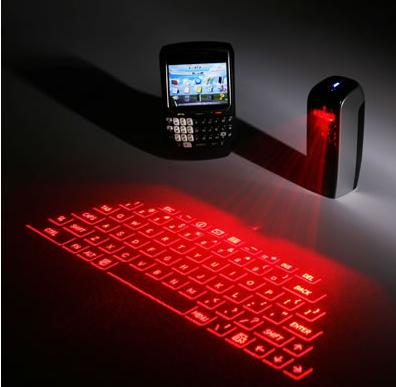
\includegraphics{celluonKeyboard.jpg}
Figure 1
\cite{image}

\pagebreak

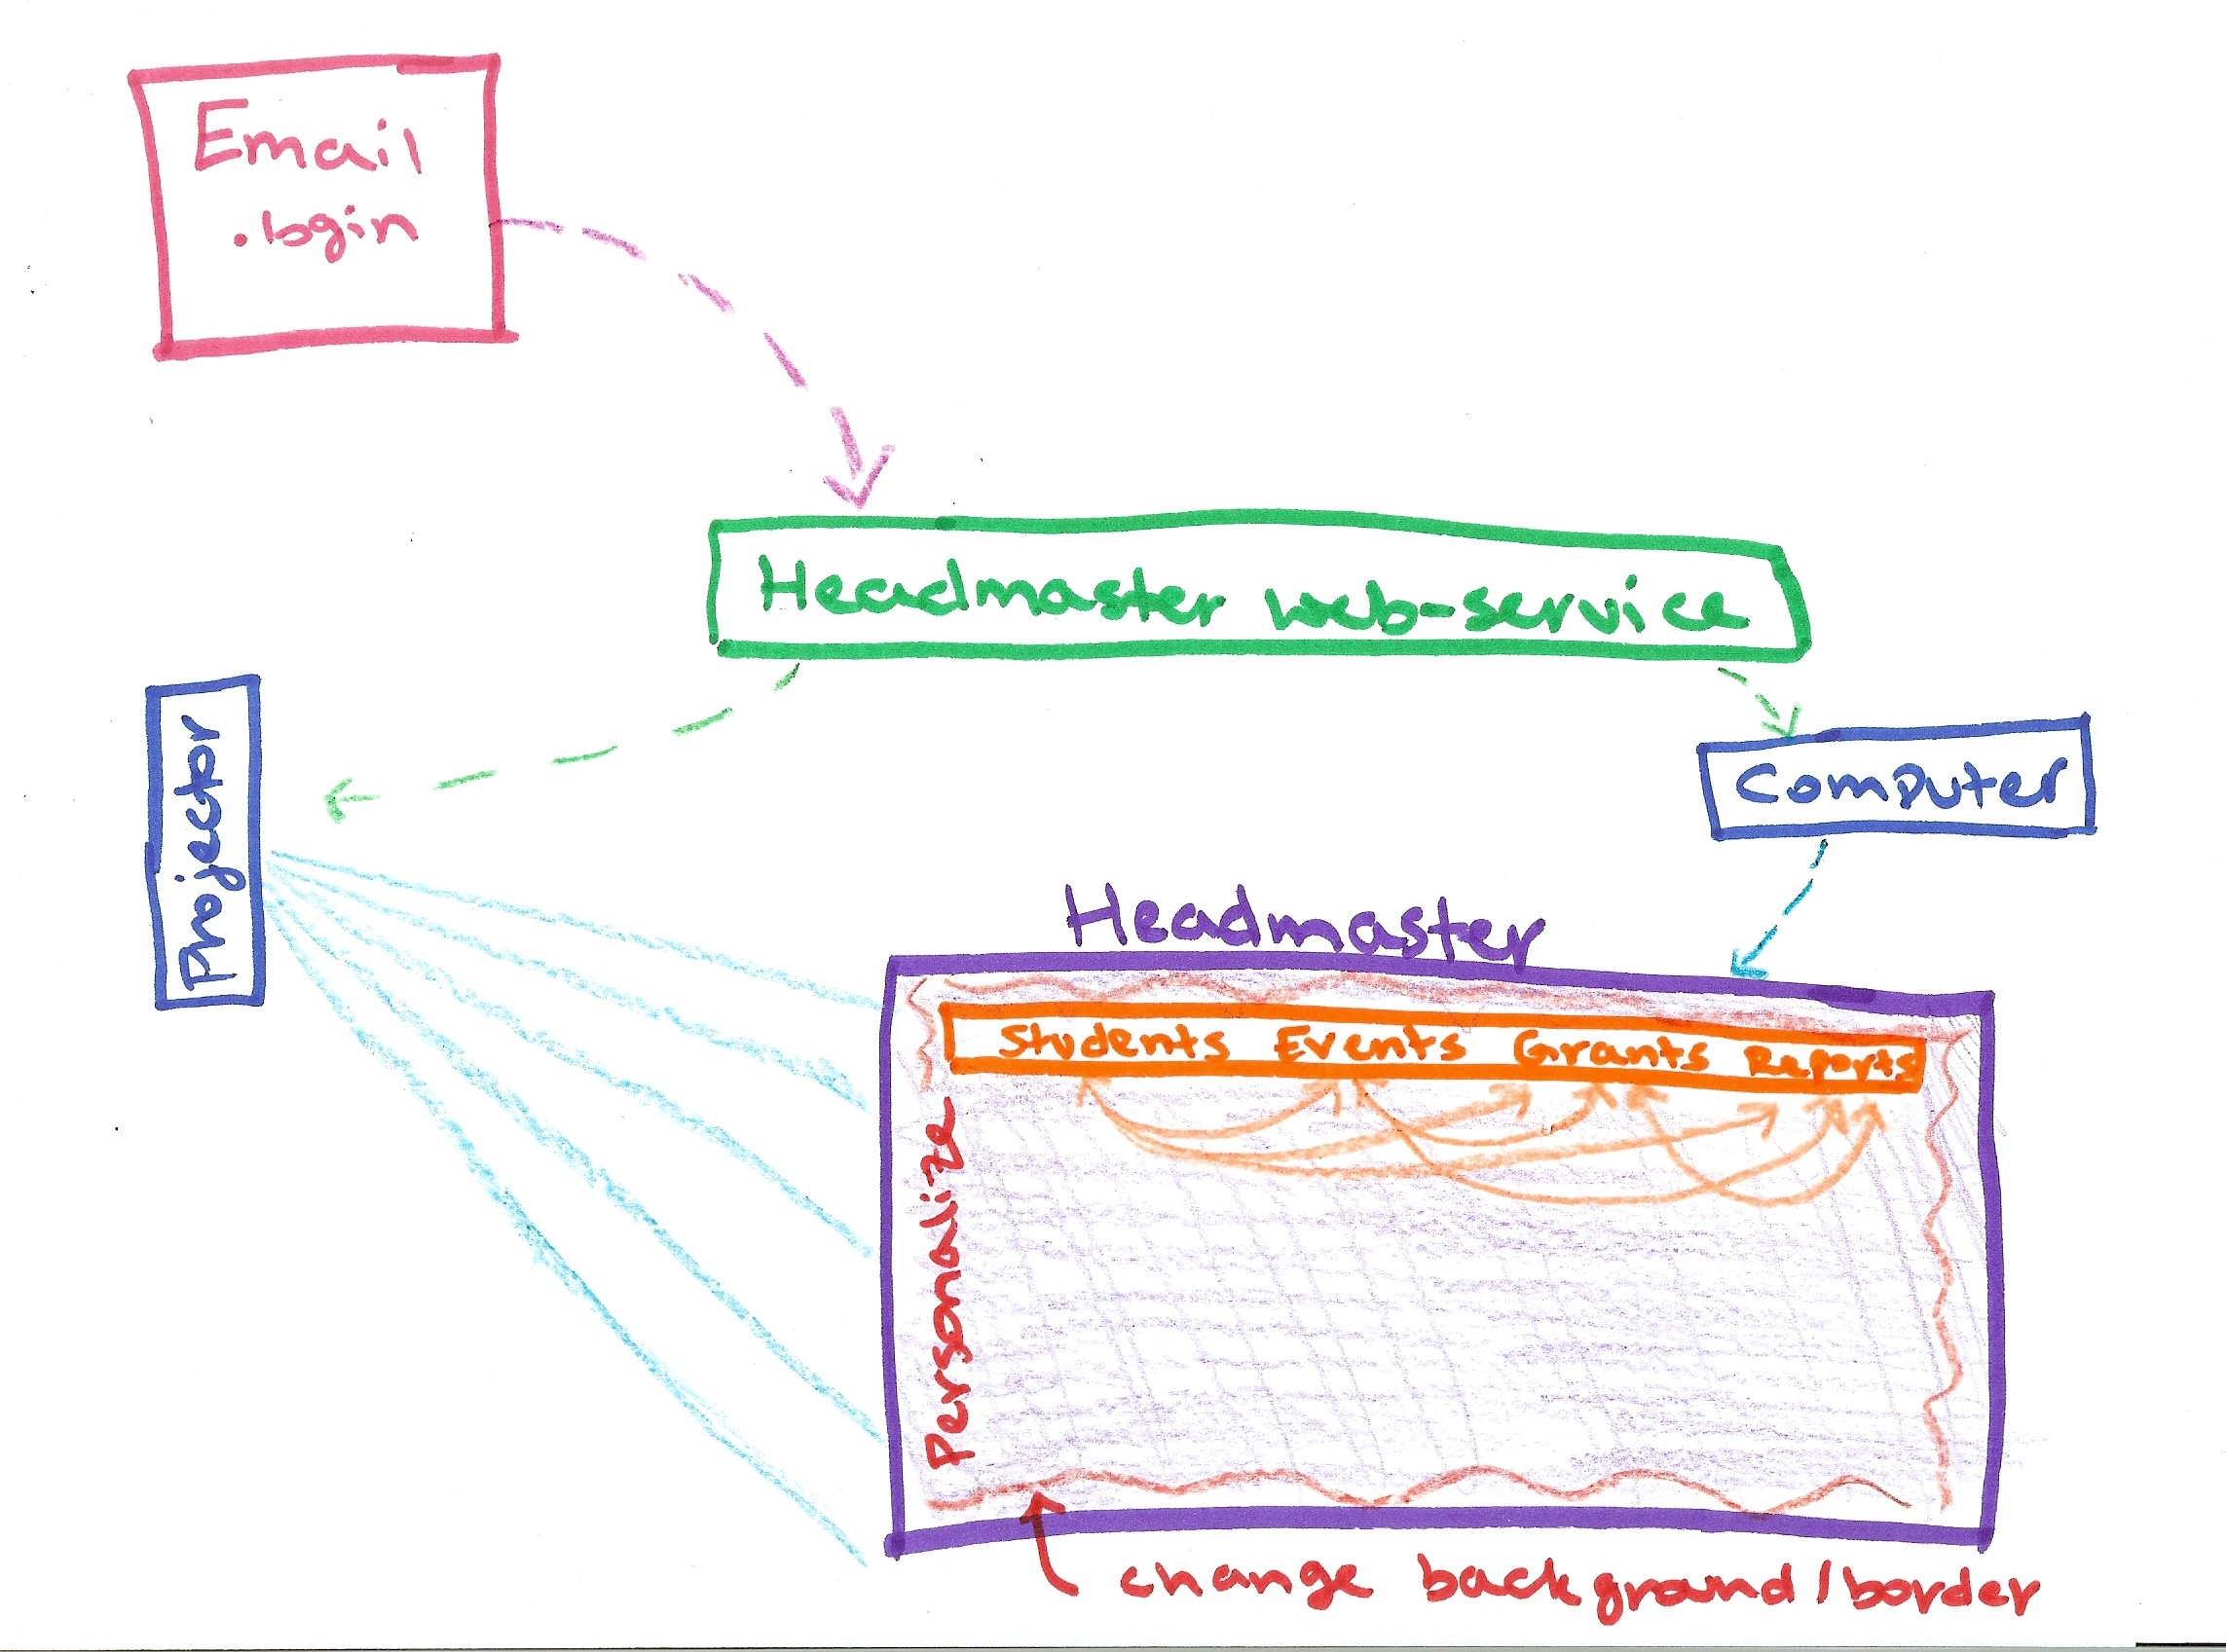
\includegraphics[scale=.50]{interfaceDesign.jpg}

Figure 2

\end{document}
